\chapter{Resultados}

En este capítulo se presentan los resultados obtenidos de la ejecución del proyecto bajo ciertas condiciones representativas, con la intención de validar la funcionalidad y también de encontrar los puntos fuertes y las falencias del mismo.

\section{Configuración del Hardware}

\begin{center}
	\begin{longtable}{|l|p{4.75in}|} \hline
		\textbf{Feature} & \textbf{Description} \\ \hline
		FPGA & \begin{itemize}
			\item Cyclone II EP2C35F672C6 with EPCS16 16-Mbit serial configuration device.
			\end{itemize} \\ \hline
		I/O Interfaces &     \begin{itemize}
					\item Built-in USB-Blaster for FPGA configuration
    					\item Line In/Out, Microphone In (24-bit Audio CODEC)
   					\item Video Out (VGA 10-bit DAC)
   					\item Video In (NTSC/PAL/Multi-format)
   					\item RS232
    					\item Infrared port
   					\item PS/2 mouse or keyboard port
    					\item 10/100 Ethernet
   					\item USB 2.0 (type A and type B)
    					\item Expansion headers (two 40-pin headers)
				     \end{itemize} \\ \hline
		Memory & \begin{itemize}
					\item 8 MB SDRAM, 512 KB SRAM, 4 MB Flash
    					\item SD memory card slot
    			 \end{itemize} \\ \hline
		Displays & \begin{itemize}
					\item Eight 7-segment displays
    					\item 16 x 2 LCD display
    			 \end{itemize} \\ \hline
		Switches and LEDs & \begin{itemize}
					\item 18 toggle switches
    					\item 18 red LEDs
   					\item 9 green LEDs
   		 			\item Four debounced pushbutton switches
   				     \end{itemize} \\ \hline
		Clocks & \begin{itemize}
					\item 50 MHz clock
    					\item 27 MHz clock
   					\item External SMA clock input
   			 \end{itemize}	 \\ \hline
	\end{longtable} 
\end{center}

La FPGA incluida en la placa es una Cyclone II EP2C35 cuyas especificaciones son:

\begin{center}
	\begin{longtable}{|l|p{1.75in}|} \hline
		\textbf{Feature} & \textbf{Description} \\ \hline
		LEs & 33216 \\ \hline
		Total RAM bits & 483840 \\ \hline
		Embedded multipliers & 35 \\ \hline
		PLLs & 4 \\ \hline
		Maximum user I/O pins & 475 \\ \hline
	\end{longtable}
\end{center}

\subsection{Caso loopback}
\begin{figure}[h]
  \centering
	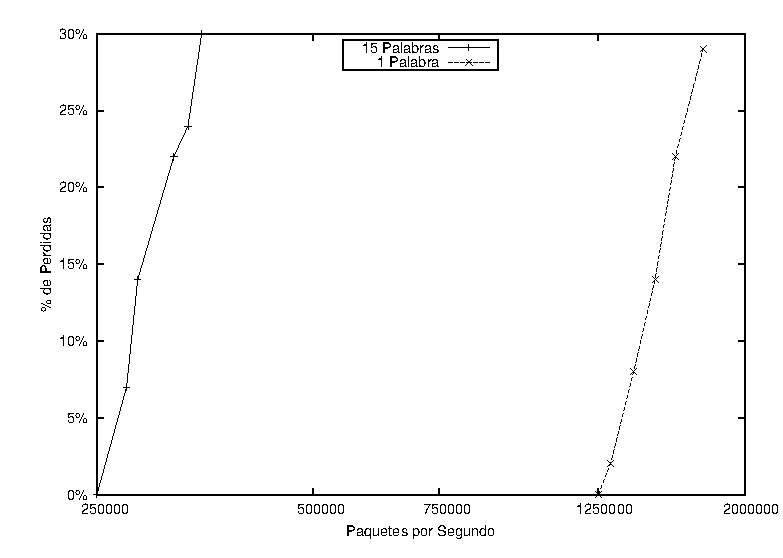
\includegraphics[width=0.70\textwidth]{5-resultados/graf/loop.eps}
  \caption{Caso Loopback para 1 y 15 palabras}
  \label{fig}
\end{figure}
En primera instancia nos ocupamos del caso loopback a los fines de encontrar los limites superiores de nuestro dise\~no.  En este caso, el software solo se limita a recibir los datos e inmediatamente después confirma el procesamiento y envía los resultados de regreso al hardware. Se realizan las pruebas correspondientes para las dos versiones de Uplink.
En el eje de las abscisas es posibles ver la cantidad de paquetes por segundo, el origen corresponde a la mayor velocidad a la que es posible transmitir sin perdidas. En las Ordenadas se puede observar la cantidad de paquetes perdidos en valores porcentuales, para obtener esta métrica se proceso una cantidad constante de paquetes, 9000, y luego se contrasto este valor con un contador global que el Generador estampa en la ultima palabra de cada paquete. Así se calculo la cantidad paquetes perdidos, sobre la cantidad total de paquetes generados. Este mismo sistema es el usado en todos los gráficos posteriores.

\subsection{Caso Algoritmos únicamente}

Se estudiará la performance de los algoritmos aplicados, midiendo el retardo de lookup en función de la posición en la tabla de ruteo, se realizaran las pruebas de manera independiente al modulo extracto de cabeceras, para así obtener una medida mas exacta del rendimiento.

\begin{figure}[h]
  \centering
	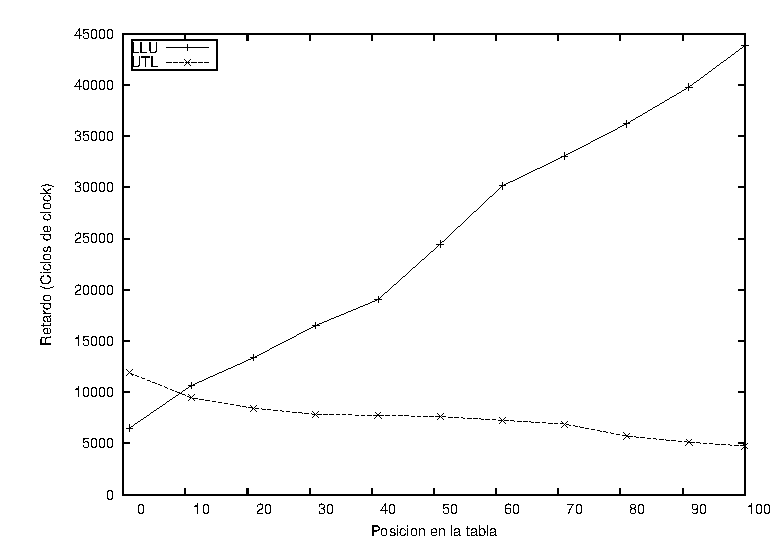
\includegraphics[width=0.8\textwidth]{5-resultados/graf/llu-utlsof.eps}
  \caption{Retardo de Búsqueda LLU vs UTL}
  \label{fig}
\end{figure}

\subsection{Completa.}

Se verificara el rendimiento del sistema implementado de manera completa. Para conseguir gráficos representativos se seleccionaran tres puntos en las curvas que indican los tiempos de accesos del algoritmos, un punto mínimo que corresponde al menor tiempo de acceso para el algoritmo en cuestión, un punto promedio que ejercita 10 entradas equidistantes a lo largo de la tabla y un punto máximo que indica el peor acceso posible. 

\subsubsection{Linear Lookup}


\begin{figure}[!h]
  \centering
	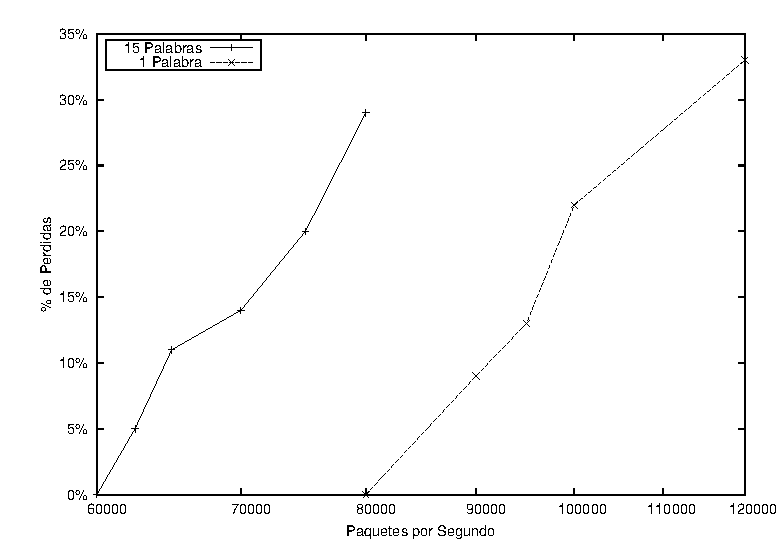
\includegraphics[width=0.7\textwidth]{5-resultados/graf/llumin.eps}
  \caption{Retardo Mínimo LLU}
  \label{fig}
\end{figure}
\begin{figure}[!h]
  \centering
	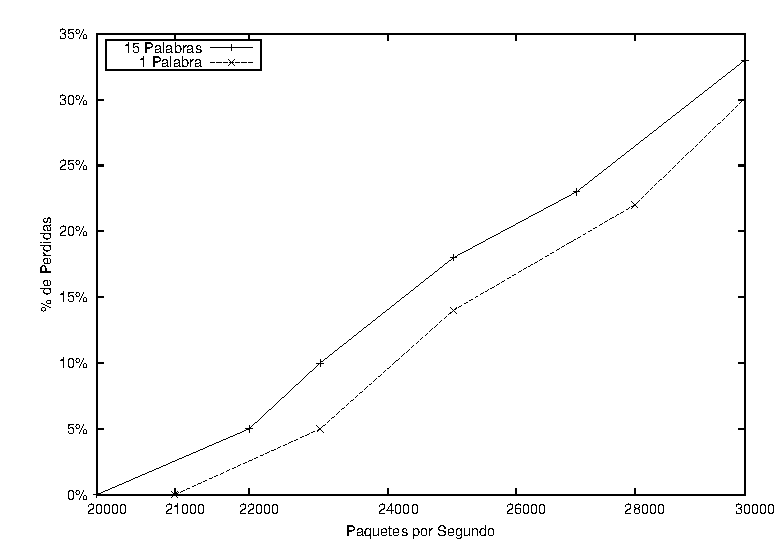
\includegraphics[width=0.7\textwidth]{5-resultados/graf/lluprom.eps}
  \caption{Retardo promedio LLU}
  \label{fig}
\end{figure}
\begin{figure}[!th]
  \centering
	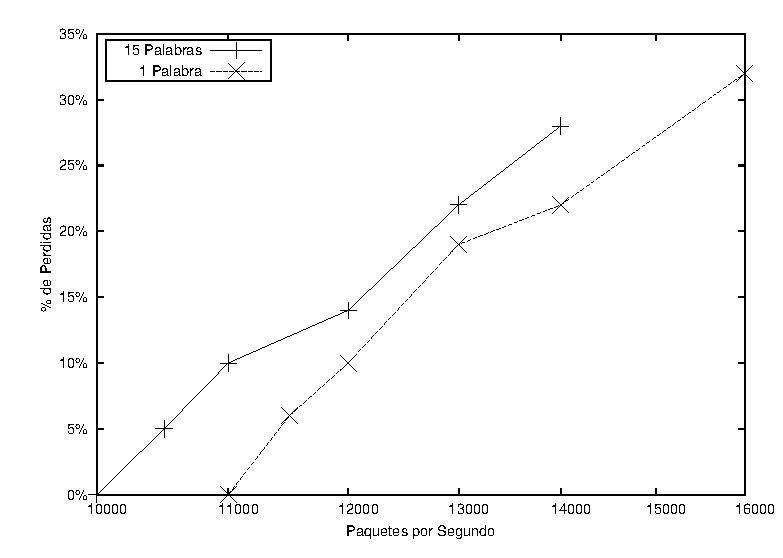
\includegraphics[width=0.7\textwidth]{5-resultados/graf/llumax.eps}
  \caption{Retardo Mínimo LLU}
  \label{fig}
\end{figure}



Se puede observar que la diferencia entre la cantidad de paquetes que pueden ser transmitidos sin errores en el mejor caso(Mínimo) entre el modulo que envía una palabra al procesador y el que envía toda la cabecera, es considerable, mientras que a medida de que se avanza en el recorrido de la tabla estos valores convergen, lo que era esperable ya que para accesos muy lentos a la tabla, el retardo introducido por el Hardware se vuelve despreciable.

\newpage
\subsubsection{Unibit Trie Lookup}

En los gráficos que corresponden al Unibit trie LookUp se puede observar que existe una menor diferencia entre la máxima cantidad de paquetes que es posible transmitir sin error en cada uno de los 3 puntos elegidos. Así como también la diferencia entre enviar el paquete entero y solo la IP destino se vuelve mas imperceptible, lo que da la pauta de que a medida de que el tiempo de acceso se vuelve mas uniforme la mejora introducida en el Hardware se vuelve despreciable.

\begin{figure}[!h]
  \centering
	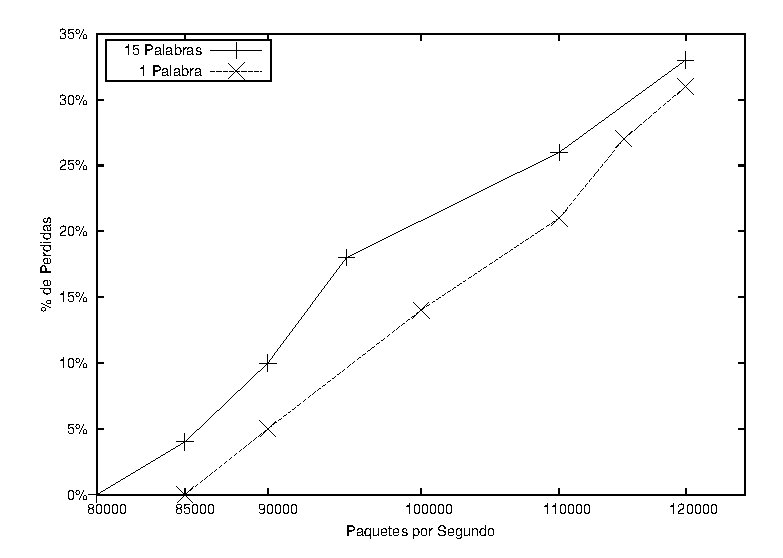
\includegraphics[width=0.7\textwidth]{5-resultados/graf/utlmin.eps}
  \caption{Retardo Mínimo UTL}
  \label{fig}
\end{figure}
\begin{figure}[!h]
  \centering
	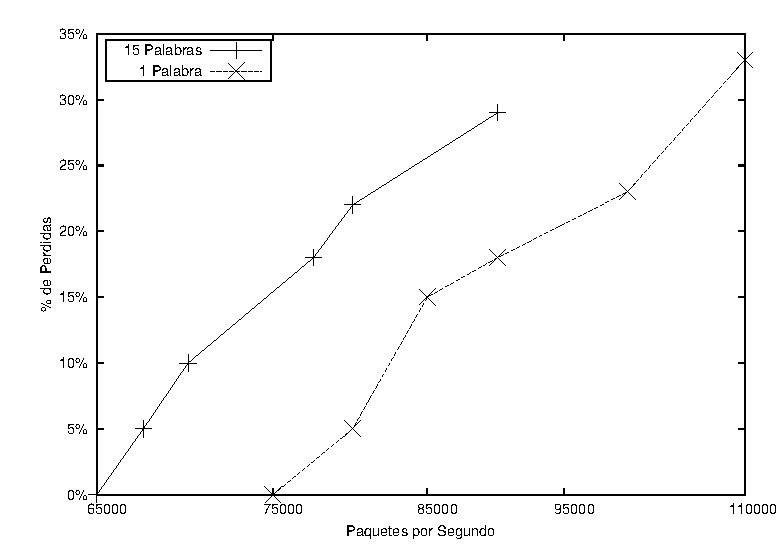
\includegraphics[width=0.7\textwidth]{5-resultados/graf/utlprom.eps}
  \caption{Retardo promedio UTL}
  \label{fig}
\end{figure}
\begin{figure}[!h]
  \centering
	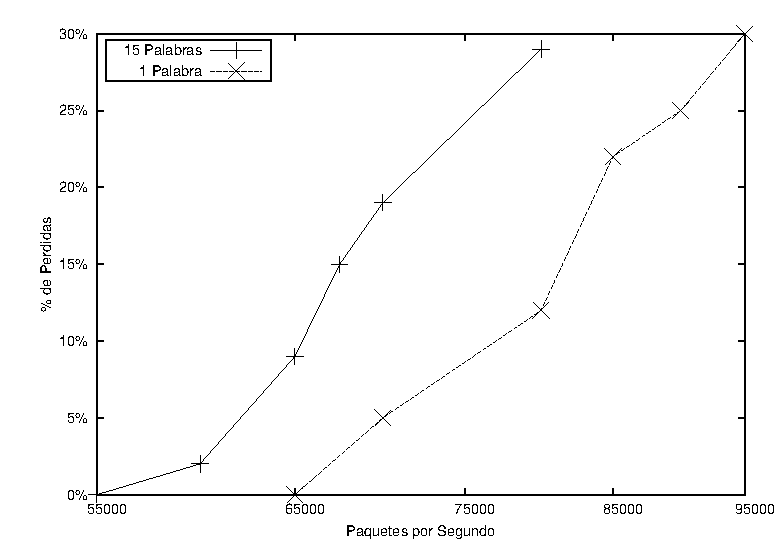
\includegraphics[width=0.7\textwidth]{5-resultados/graf/utlmax.eps}
  \caption{Retardo Mínimo UTL}
  \label{fig}
\end{figure}

\newpage
\subsection{Cache}

Se probara el funcionamiento del sistema incluyendo la cache implementada en software. Para ello, se efectuara una toma de datos en la cual se compararan 2 sucesiones: la primera de ella resultara en fallos al no estar presente ninguno de los valores.

Puede notarse que, en el caso de que la búsqueda termine en un miss, se introduce un retardo adicional (si se compara con el escenario en el cual no existe la cache). Ello se debe a la búsqueda que se efectúa en la cache antes de hacerlo propiamente en la tabla de ruteo, tanto en la implementación linked-list como en la implementación unibit-trie.

